\section{Bluetooth-Modul XS3868} \label{sec:4.1}
\subsection{Allgemeines} \label{subsec:4.1.1}
Ein Audio-Bluetooth-Modul soll in einfacher Weise ein Audio-Signal von beispielsweise einem Smartphone ausgeben. Dabei ist eine hohe Kompatibilität mit viele Geräten wichtig, weil es sehr viele verschiedene Versionen von Bluetooth gibt. Da Bluetooth-Geräte meist abwärtskompatibel sind, ist es sinnvoll das Modul mit einer älteren BT-Version laufen zu lassen.


\subsection{Zielsetzung} \label{subsec:4.1.2}
Es soll ein Print angefertigt werden auf dem sich das BT-Modul samt Versorgungsschaltung befindet. Auf diesem Print wird zusätzlich noch eine Additionsschaltung vorgesehen, um auch mit einem Klinkeneingang ein Signal zuführen zu können, falls das BT-Modul ausfällt.\\
Um eine leichtere Handhabung zu ermöglichen, muss auch ein Adapterprint für das BT-Modul angefertigt werden.


\subsection{Auswahl des Bluetooth-Moduls} \label{subsec:4.1.3}
Wie bereits erwähnt soll das BT-Modul mit möglichst viele Geräten kompatibel sein, also mit einer älteren BT-Version laufen. Es sollte weiterhin eine möglichst einfache Bedienung für den Benutzer ermöglichen (beispielsweise Play-/Pausetaste).\\
Außerdem soll es bei geringen Kosten eine möglichst gute Verbindung, d.h. einen hohe Reichweite, erzielt werden.\\
Nach ausführlicher Recherche wurde das Modul \enquote{XS3868 Revision 3} ausgewählt. Der darauf verbaute Chip \enquote{OVC3860} von \enquote{OmniVision Technologies} hat sich bereits in vielen anderen Projekten bewährt. 


\newpage
\subsection{OVC3860} \label{subsec:4.1.4}
In dem Chip (Abb. \ref {fig:4.1.4.1}) ist außer der Bluetooth-Verbindung auch noch ein Stereo-Audio-Prozessor verbaut. Zusätzlich gibt es noch eine UART-Schnittstelle mithilfe man einige Einstellungen am Chip vornehmen kann. Eine kleine LiPo-Ladeschaltung ist ebenfalls vorhanden, wird aber in diesem Fall nicht verwendet.\\
Das Modul benötigt eine Versorgungsspannung von 3,3V bis 4,2V, wobei der Chip mit 1,8V versorgt wird. Diese Spannung wird auf dem Modul erzeugt.\\
Die verwendete BT-Version ist 2.0. Einige GPIO-Pins sind auf das Modul herausgeführt um Funktionen wie \enquote{Play/Pause} zu ermöglichen. Der Chip benötigt einen externen Speicher und eine Antenne (auf dem Modul) um ordnungsgemäß zu funktionieren.
\begin{figure} [H]
	\centering
	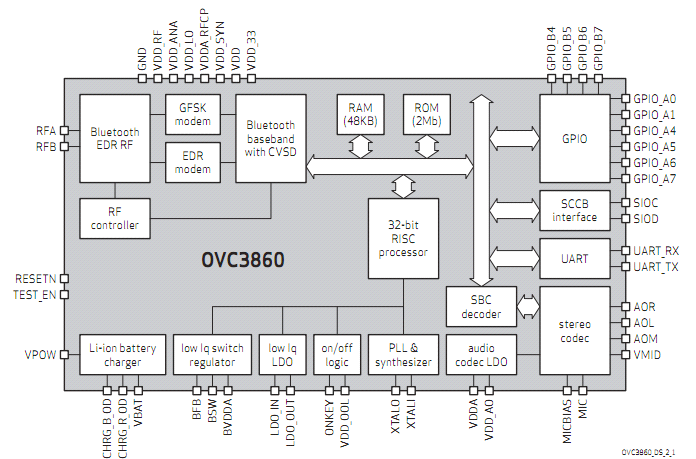
\includegraphics[width=0.8\textwidth]{img/BTModul/blockschaltbild.png}
	\caption{Blockschaltbild OVC3860}\label {fig:4.1.4.1}
\end{figure}
\newpage

\subsection{Pinbelegung} \label{subsec:4.1.5}
Insgesamt hat das Modul 23 verwendbare Pins, aufgeteilt auf 2 Seiten in 11 und 12 Pins.
\begin{figure} [H]
	\centering
	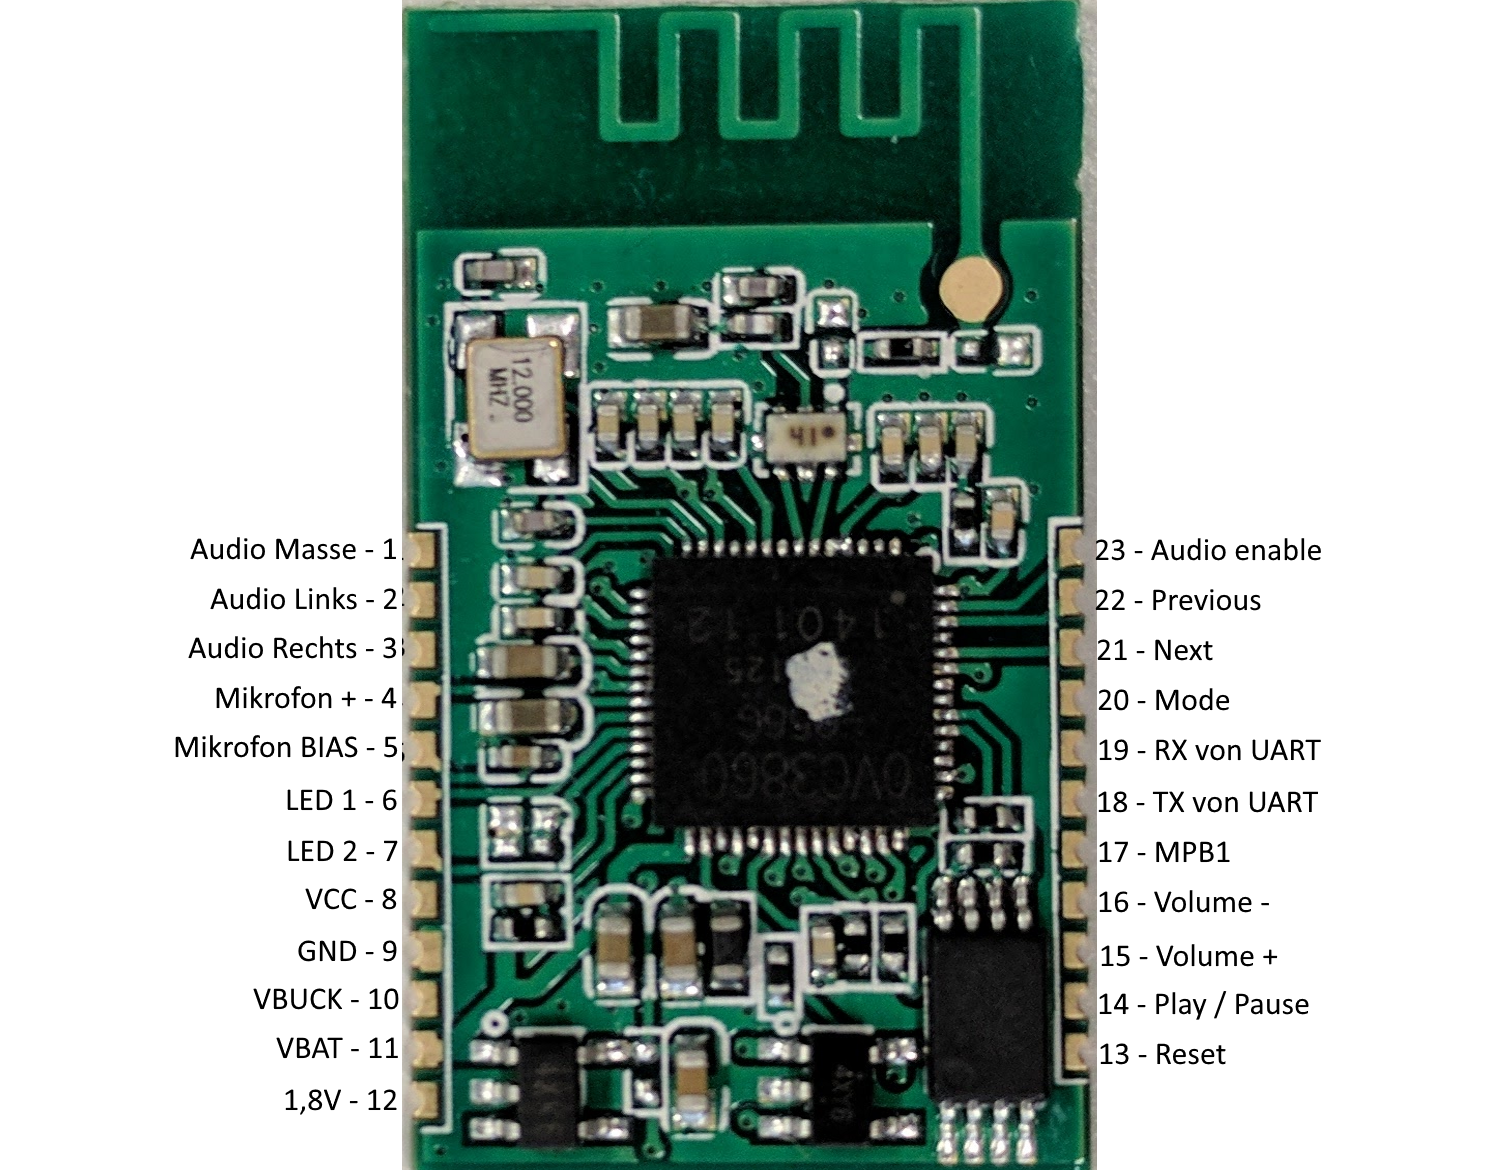
\includegraphics[width=1\textwidth]{img/BTModul/XS3868_Pinbelegung.png}
	\caption{Pinbelegung XS3868}\label {fig:4.1.5.1}
\end{figure}
Wie in Abbildung \ref{fig:4.1.5.1} dargestellt, ist der Audio-Ausgang auf den Pins 1-3. Die Status-LED für das Modul wird mit dem Pin 6 geschaltet.\\ \\
Die Versorgung des Moduls erfolgt über die Pins 11 (VBAT) und 9 (GND). Für die Audiofunktionen wird eine konstante Spannung (1,8V - Pin 12) benötigt. Diese Funktionen befinden sich auf den Pins 14-16 und 21-22. Sie werden mit Tastern beschalten.\\
Die UART-Schnittstelle befindet sich auf den Pins 18-19.\\
Außerdem verfügt das Modul auch über eine Mikrofon-Funktion, die aber in diesem Projekt nicht verwendet wird.
\newpage


\subsection{Inbetriebnahme} \label{subsec:4.1.6}
Bereits mit einer simplen Beschaltung kann das Modul in Betrieb genommen werden:
\begin{figure} [H]
	\centering
	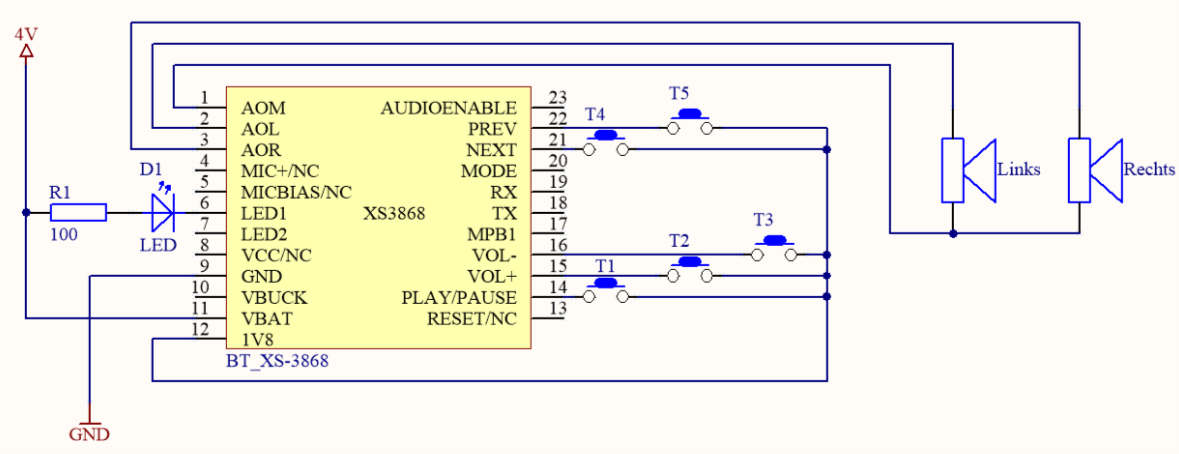
\includegraphics[width=1\textwidth]{img/BTModul/XS3868_Prinzipschaltung.png}
	\caption{Prinzipschaltung XS3868}\label {fig:4.1.6.1}
\end{figure} 
Mit dieser Schaltung (Abb. \ref {fig:4.1.6.1}) kann das Modul bereits ordnungsgemäß arbeiten.\\
Die Versorgungsspannung ist mit 4V etwas höher gewählt damit es nicht zu Ausfällen durch Spannungsschwankungen kommt. Das XS3868-Modul hat eine Stromaufnahme von ca. 30mA beim Starten, 10mA im Stand-By und bis zu 100mA wenn Musik abgespielt wird.\\ \\
Die Status-LED ist, wie in Abbildung \ref {fig:4.1.6.1} dargestellt, \enquote{Low-Aktiv}. Beim Starten des Moduls und während der Suche nach Geräten blinkt sie durchgehend, wobei sie bei einer bestehenden Verbindung nur die Hälfte der Zeit blinkt.\\ \\
Mit einfachem Betätigen eines Tasters wird die entsprechende Funktion vom Modul ausgeführt, jeweils mit einem Bestätigungston begleitet. Dieser Ton wird auch beim Starten des Moduls abgespielt.\\ \\
Statt die Lautsprecher direkt an das Modul anzuschließen, sollte allerdings noch ein Verstärker verbaut werden.
\newpage


\subsection{Verbindung mit dem Modul} \label{subsec:4.1.7}
Wenn der OVC3860 eingeschaltet ist, sucht er andauernd nach BT-Geräten. Mit einem Smartphone findet man das Gerät und kann sich mit einem Standard-PIN-Code (\enquote{0000}) verbinden. Wenn bereits Lautsprecher angeschlossen sind, wird ein Ton abgespielt, der die Verbindung bestätigt. Außerdem hat die Status-LED nun ein anderes Blinkverhalten (Mehrmaliges Blinken mit längeren Pausen).\\
Jetzt ist das Modul bereit Musik abzuspielen. Diese kann vom Smartphone oder vom Modul aus gesteuert werden. Die notwendigen Taster müssen allerdings schon in der Schaltung verbaut sein um die Bedienung der Musik zu ermöglichen.


%\section{Zusatz-Leiterplatten} \label{sec:4.3}
%\subsection{Allgemeines} \label{subsec:4.3.1}
%Als Entwicklungsprogramm für beide Leiterplatten wurde  \enquote{Altium Designer 13.3} verwendet. Die Schaltung wurde in diesem Programm gezeichnet, das Layout für die Leiterplatten angefertigt und entflechtet. Es wurden einseitige Platinen verwendet, da doppelseitige nicht notwendig waren.


\subsection{Adapter-Board} \label{subsec:4.1.8}
Da das Modul in SMD-Bauform gefertigt ist, wurde ein Adapter-Board (Abb. \ref{fig:4.1.8.1}) vorgesehen um eine einfachere Handhabung mit dem Modul zu ermöglichen. Als Anschlussmöglichkeiten werden Stiftleisten verwendet.\\
Die Schaltung ist deshalb auch sehr simpel aufgebaut:
\begin{figure} [H]
	\centering
	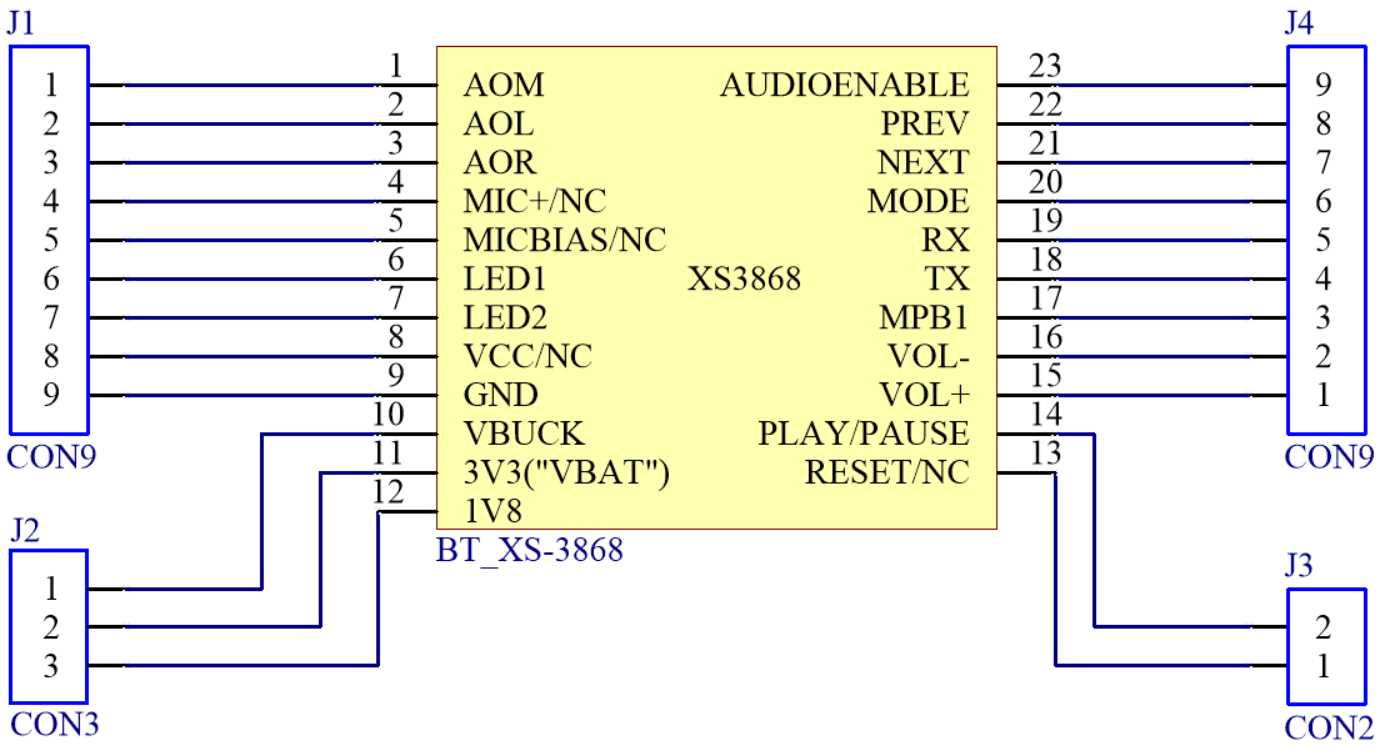
\includegraphics[width=1\textwidth]{img/BTModul/adapter_sch.png}
	\caption{Schaltung des Adapter-Boards}\label {fig:4.1.8.1}
\end{figure} 
Jeder Pin bekommt auch auf dem Adapter einen eigenen Pin auf der Stiftleiste.
\newpage
Das PCB (Abb. \ref{fig:4.1.8.2}) ist, wie bereits erwähnt, einseitig aufgebaut:
\begin{figure} [H]
	\centering
	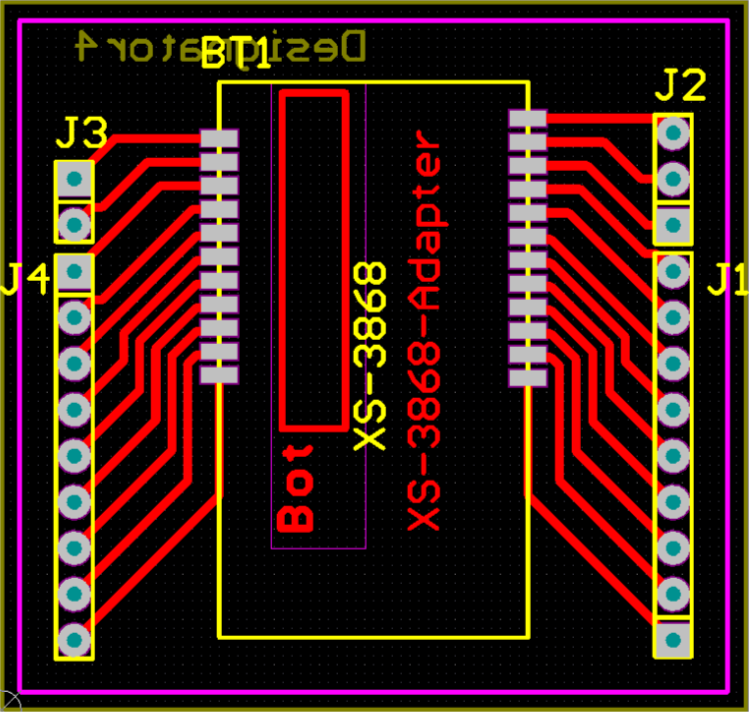
\includegraphics[width=1\textwidth]{img/BTModul/adapter_pcb.png}
	\caption{PCB des Adapter-Boards}\label {fig:4.1.8.2}
\end{figure} 
Mit diesem PCB kann da BT-Modul nun besser getestet und auch weiterverwendet werden. Gemeinsam mit diesem Adapter kommt es auch auf das Hauptboard.
\newpage


\subsection{Hauptboard} \label{subsec:4.1.9}
\subsubsection{Funktion} \label{subsubsec:4.1.9.1}
Das Hauptboard wird hauptsächlich zur Versorgung des BT-Moduls, aber auch zur Weiterverarbeitung des Audio-Signals verwendet. Darüber hinaus ist eine Additionsschaltung vorgesehen, die das Signal des BT-Moduls mit einem zweiten, von einem Klinken-Eingang zugeführten, Signal vermischt. Die Lautstärke von diesem zweiten Audio-Signal kann über ein Stereo-Potentiometer geregelt werden. \\
Weiterhin sind die Pins zur Bedienung der Musik an einen 2x5-Wannenstecker herausgeführt. Zugang zur seriellen Schnittstelle wird auch ermöglicht.

\subsubsection{Schaltung} \label{subsubsec:4.1.9.2}
Die Schaltung (Abb. \ref{fig:4.1.9.2.1}) des Hauptboards ist in mehrere Teile aufgeteilt und wird deshalb auch einzeln erklärt.
\begin{figure} [H]
	\centering
	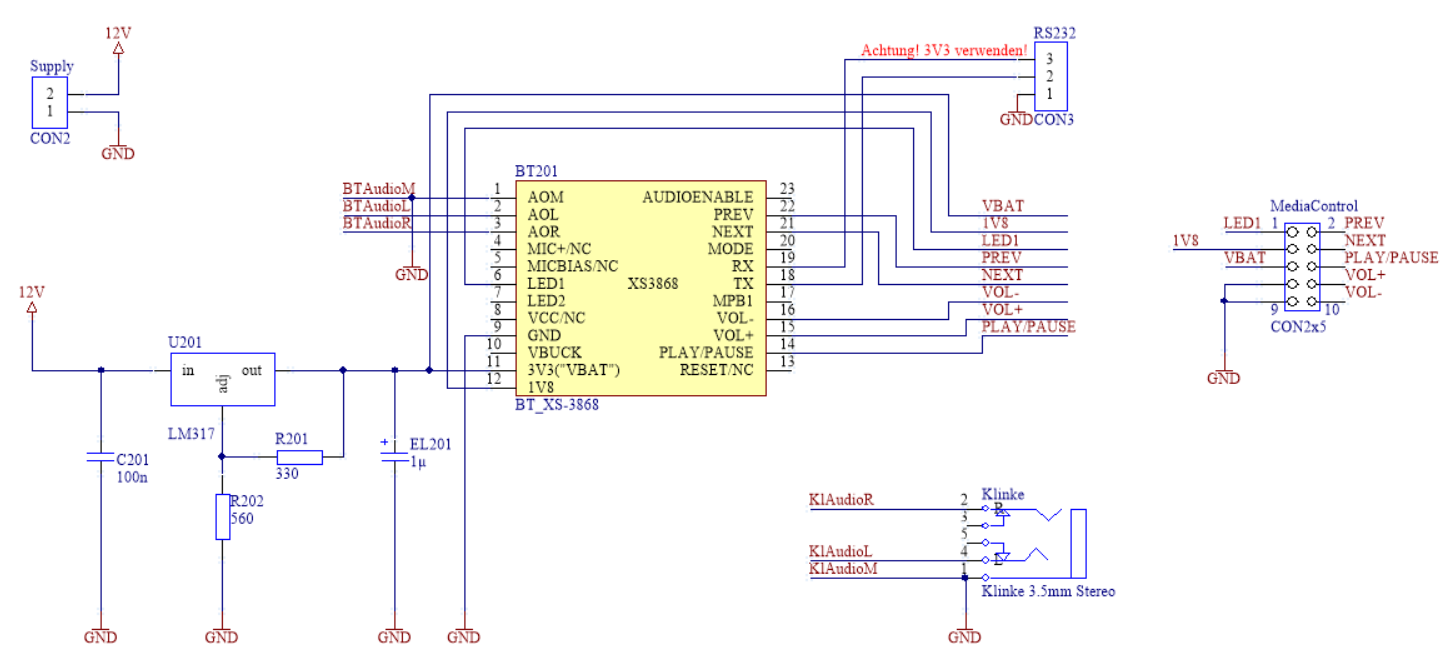
\includegraphics[width=1\textwidth]{img/BTModul/hauptboard_sch1.png}
	\caption{Schaltung des Hauptboards (Versorgung + BT-Modul)}\label {fig:4.1.9.2.1}
\end{figure} 
In diesem Teil der Schaltung ist zu sehen: die Versorgungsbuchse, die Versorgungsschaltung für das BT-Modul, das BT-Modul mit herausgeführten Pins und die Klinken-Buchse.\\
Der Spannungsregler LM317 (Bezeichnung: U201) stellt eine Versorgungsspannung von 3,9V für das BT-Modul ein. Mit einer maximalen Stromaufnahme von 100mA ergibt sich folgende Verlustleistung:
\begin{equation}
	P_{max} = 8,1V * 100mA = 0,81W
\end{equation}
Deshalb wird auch kein Kühlkörper benötigt, es wird aber trotzdem eine Alu-Platte an den LM317 geschraubt um sicher zu gehen. \\
Ein eigener Stecker (Stiftleiste) für die Versorgung (12V) sowie die UART-Schnittstelle (RS232) sind auch vorgesehen. Der Wannenstecker (hier: \enquote{MediaControl}) ist mit allen wichtigen Pins des Moduls verbunden und verbindet eine Frontplatine mit dem Hauptboard. \\
Die Klinkenbuchse wird in der folgenden Additionsschaltung(Abb. \ref {fig:4.1.9.2.2}) weiterverwendet:
\begin{figure} [H]
	\centering
	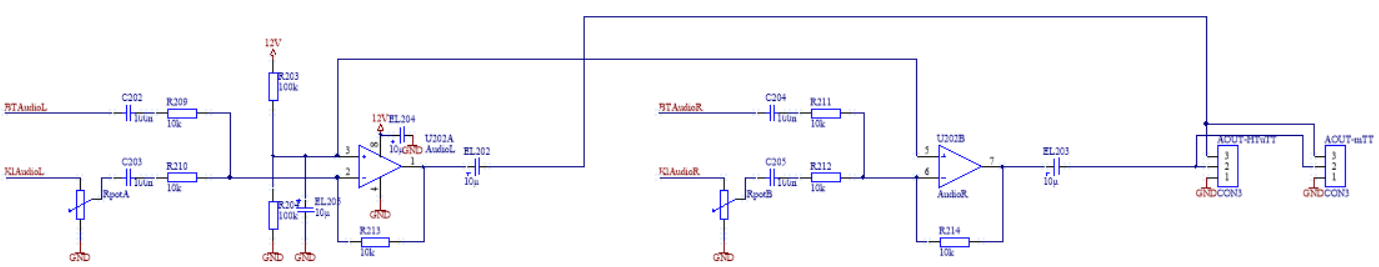
\includegraphics[width=1\textwidth]{img/BTModul/hauptboard_sch2.png}
	\caption{Schaltung des Hauptboards (Additionsschaltung)}\label {fig:4.1.9.2.2}
\end{figure}
Vergrößert:
\begin{figure} [H]
	\centering
	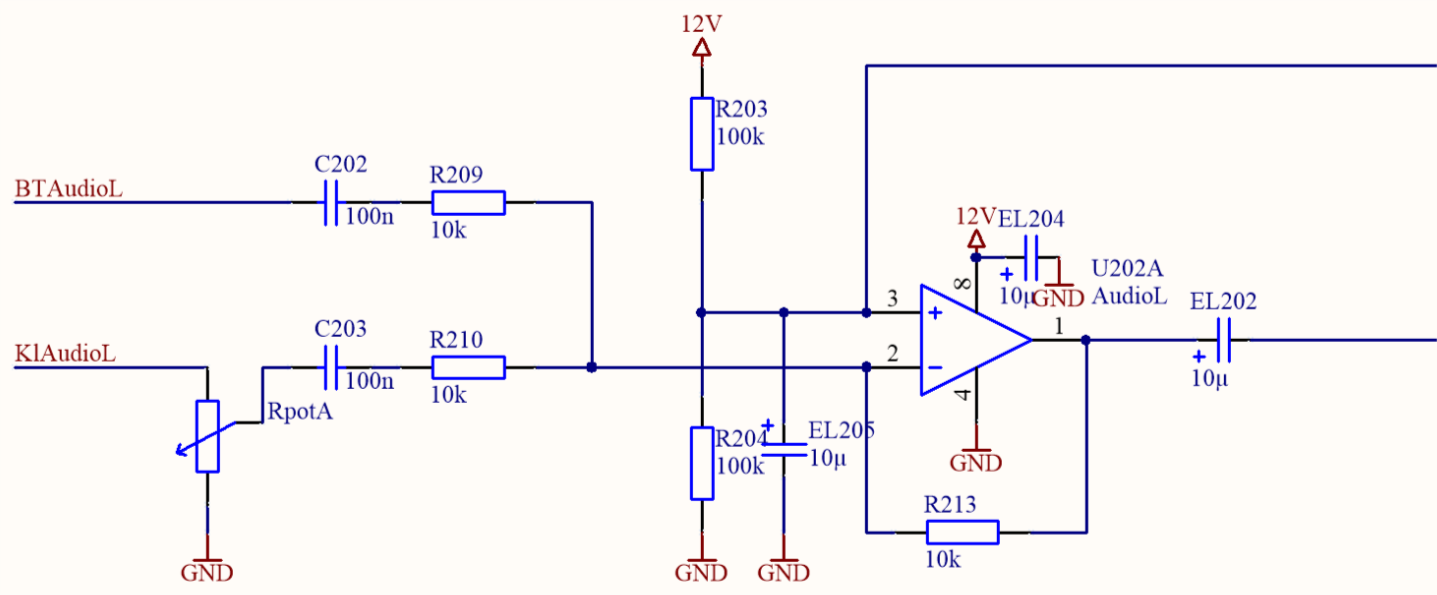
\includegraphics[width=1\textwidth]{img/BTModul/hauptboard_sch2_zoom.png}
	\caption{Schaltung des Hauptboards (linker Teil der Additionsschaltung)}
\end{figure}
Mithilfe dieser OPV-Schaltung werden die zwei Audio-Signale (ein Addierer pro Kanal) addiert. Das Signal vom Klinkeneingang kann zuvor noch mit einem Potentiometer abgeschwächt werden.\\
Der Arbeitspunkt bei 6V am Pin 3 wird benötigt um am Ausgang eine Spannung von $\pm$6V zu erreichen. Der OPV wird hier als invertierender Verstärker mit Verstärkung 1 aufgebaut, aber er addiert hier die zwei Signale zusammen auf ein Ausgangssignal.

\subsubsection{PCB} \label{subsec:4.1.9.3}
Die Platine(Abb. \ref {fig:4.1.9.3.1}) für das Hauptboard sollte möglichst kompakt sein und alle Eingänge oder Bedienelemente auf einer Seite (hier rechts) haben. Das BT-Modul wird samt Adapter auf zwei Stiftleisten gesteckt. Darunter werden keine Bauteile verwendet, weil es sonst zu eng wäre. Des weiteren wären Bauteile unter dem Adapterprint während der Testphase unvorteilhaft, da diese schwerer zugänglich sind.
\begin{figure} [H]
	\centering
	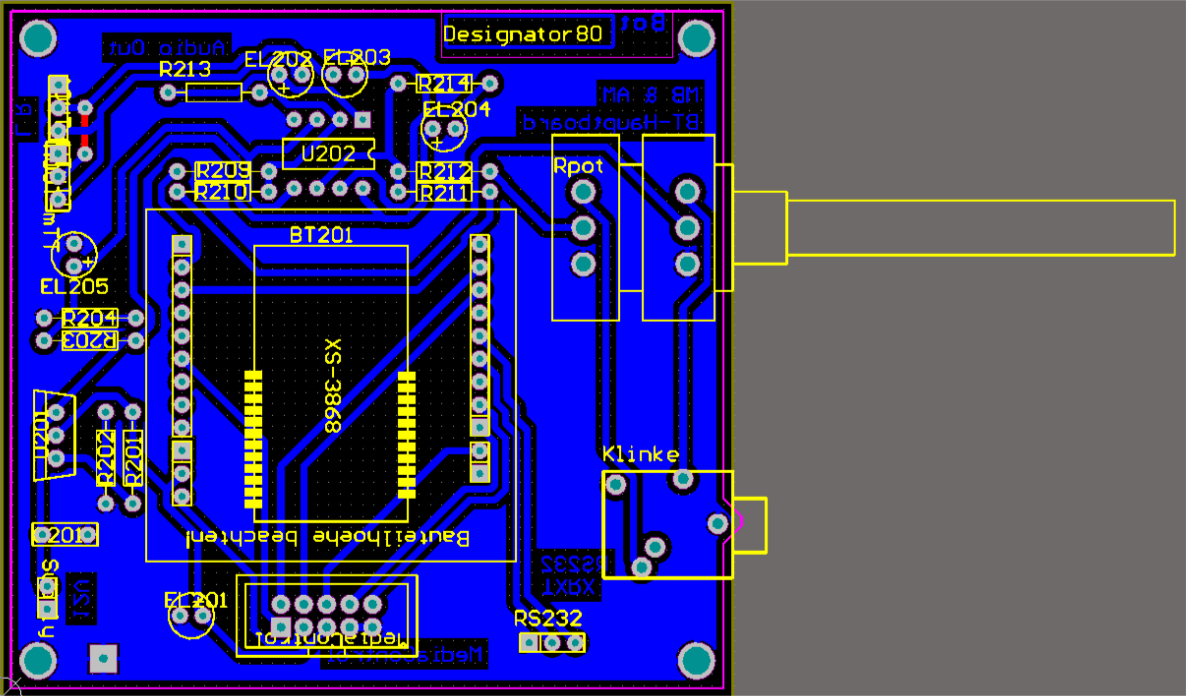
\includegraphics[width=1\textwidth]{img/BTModul/hauptboard_pcb.png}
	\caption{PCB des Hauptboards}\label {fig:4.1.9.3.1}
\end{figure}
\newpage


\subsection{Frontplatine} \label{subsec:4.1.10}
\subsubsection{Funktion} \label{subsubsec:4.1.10.1}
Diese Platine ist eigentlich eine Erweiterung des Hauptboards. Es wird mit dem Hauptboard über einen 2x5-Wannenstecker verbunden und auch versorgt. Sonst sind nur die Taster zur Bedienung des BT-Moduls, sowie die Status-LED verbaut.

\subsubsection{Schaltung} \label{subsubsec:4.1.10.2}
Die Taster werden jeweils mithilfe eines Kondensators entprellt. Die Höhe der Taster reicht über die Kondensatoren hinaus um eine Bedienung zu ermöglichen. (Abb. \ref{fig:4.1.10.2.1})
\begin{figure} [H]
	\centering
	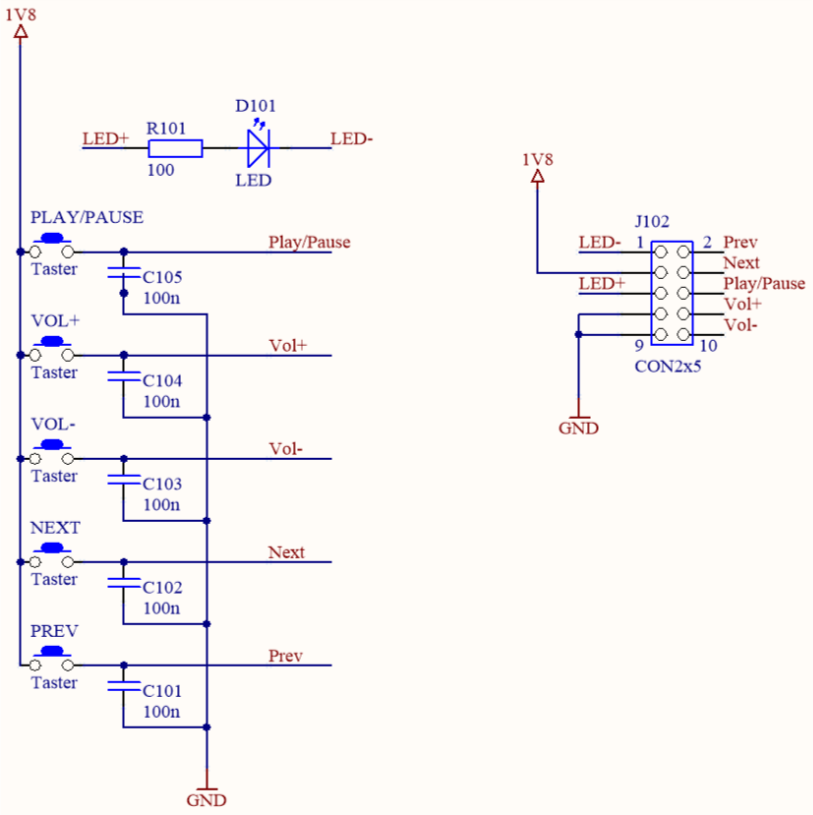
\includegraphics[width=0.7\textwidth]{img/BTModul/front_sch.png}
	\caption{Schaltung der Frontplatine}\label {fig:4.1.10.2.1}
\end{figure}
Jeder der Taster ist mit dem 1,8V-Pin des Moduls verbunden und geht dann weiter auf den entsprechenden Funktionspin. Die Bezeichnung \enquote{LED+} entspricht der Versorgungsspannung (\enquote{VBAT} = 3,9V) des Moduls. \enquote{LED-} ist mit dem Ansteuerungssignal am BT-Modul verbunden (Pin 6).

\subsubsection{PCB} \label{subsubsec:4.1.10.3}
Das PCB (Abb. \ref {fig:4.1.10.3.1}) der Frontplatine soll ebenfalls so klein wie möglich aber von der Bedienung her sinnvoll aufgebaut sein.
\begin{figure} [H]
	\centering
	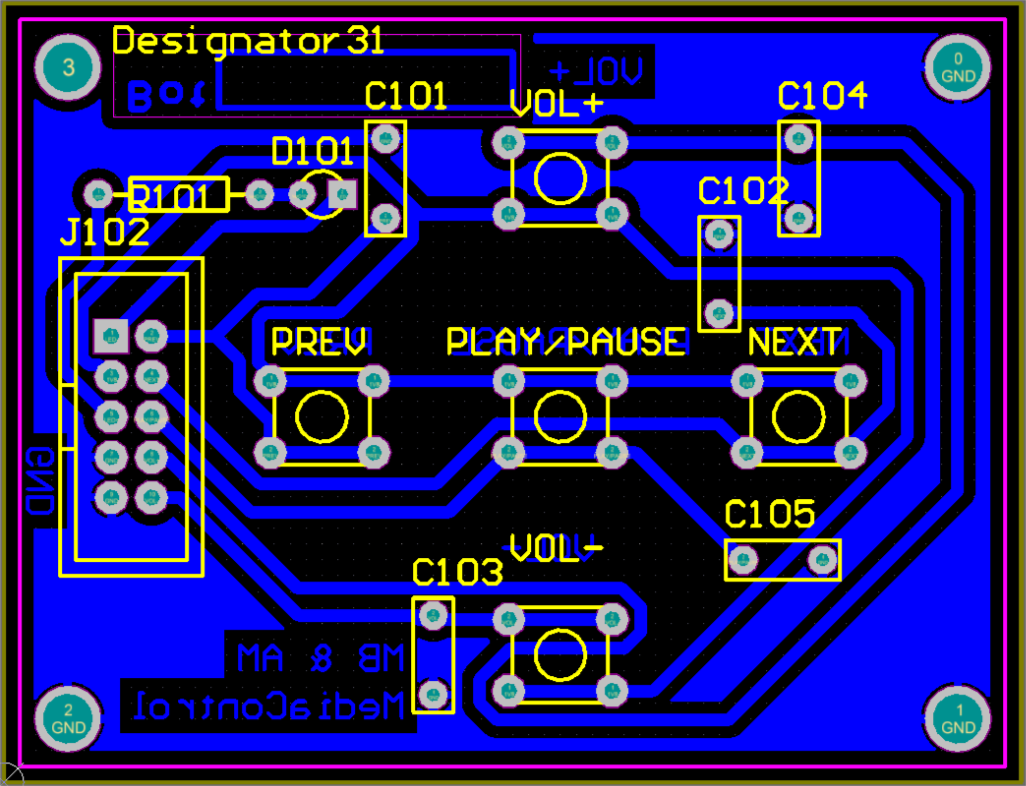
\includegraphics[width=1\textwidth]{img/BTModul/front_pcb.png}
	\caption{PCB der Frontplatine}\label {fig:4.1.10.3.1}
\end{figure}
Die Taster wurden in einem Kreuz aufgebaut, wobei an der linken oberen Ecke die Status-LED verbaut wurde.







